\documentclass[]{article}

% Imported Packages
%------------------------------------------------------------------------------
\usepackage{amssymb}
\usepackage{amstext}
\usepackage{amsthm}
\usepackage{amsmath}
\usepackage{enumerate}
\usepackage{fancyhdr}
\usepackage[margin=1in]{geometry}
\usepackage{graphicx}
%\usepackage{extarrows}
%\usepackage{setspace}
%\usepackage{xcolor}
\usepackage{color}
%------------------------------------------------------------------------------

% Header and Footer
%------------------------------------------------------------------------------
\pagestyle{plain}  
\renewcommand\headrulewidth{0.4pt}                                      
\renewcommand\footrulewidth{0.4pt}                                    
%------------------------------------------------------------------------------

% Title Details
%------------------------------------------------------------------------------
\title{Deliverable \#1 Template : Software Requirement Specification (SRS)}
\author{SE 3A04: Software Design II -- Large System Design}
\date{}
                            
%------------------------------------------------------------------------------

% Document
%------------------------------------------------------------------------------
\begin{document}

\maketitle	
\noindent{\bf Tutorial Number:} T03\\
{\bf Group Number:} G06 \\
{\bf Group Members:} 
\begin{itemize}
	\item Virochaan Ravichandran Gowri
	\item Alex Yoon
	\item Noah Goldschmied
	\item Krish Dogra
	\item Leo Vugert
\end{itemize}

\section*{IMPORTANT NOTES}
\begin{itemize}
	\item Be sure to include all sections of the template in your document regardless whether you have something to write for each or not
	\begin{itemize}
		\item If you do not have anything to write in a section, indicate this by the \emph{N/A}, \emph{void}, \emph{none}, etc.
	\end{itemize}
	\item Uniquely number each of your requirements for easy identification and cross-referencing
	\item Highlight terms that are defined in Section~1.3 (\textbf{Definitions, Acronyms, and Abbreviations}) with \textbf{bold}, \emph{italic} or \underline{underline}
	\item For Deliverable 1, please highlight, in some fashion, all (you may have more than one) creative and innovative features. Your creative and innovative features will generally be described in Section~2.2 (\textbf{Product Functions}), but it will depend on the type of creative or innovative features you are including.
\end{itemize}

\newpage
\section{Introduction}
\label{sec:introduction}
% Begin Section

\begin{itemize}
	\item Provide an overview of the document/SRS.
\end{itemize}


\subsection{Purpose}
\label{sub:purpose}
% Begin SubSection
This Software Requirement Specification has been created to specify the requirements needed to develop a secure communication app (VanklComm) for our organization. This SRS will ensure to cover functional requirements specifying how the app will perform the secure communication, including viewpoints from stakeholders and common business events and use cases and non-functional requirements outlining specifications of the system. Red text indicates a creative feature that goes beyond the project specifications.
% End SubSection

\subsection{Scope}
\label{sub:scope}
% Begin SubSection
\par The software product that will be produced is VanklComm, a secure chat application on Android. The product will allow for all employees of a company to communicate in a secure fashion, while also storing all texts in a database for security.
\\
\par \noindent Users will be required to create an account on VanklComm and be verified by their company in order to begin chatting. The main function of the product is the person-to-person chat, however there will also be \textcolor{red}{announcement boards} that managers can use to notify all of their employees.
\\
\par \noindent An objective of the software is to provide companies with secure chatting that prevents espionage from employees. Another objective of the software is that it must be easy to use, so that employees will have an easy transition over to the service. The last objective of the software is the encryption service. The software will provide end-to-end encryption on messages sent and received, which is what provides the secure chat.

% End SubSection

\subsection{Definitions, Acronyms, and Abbreviations}
\label{sub:definitions_acronyms_and_abbreviations}
% Begin SubSection
\begin{itemize}
	\item API – Application Programming Interface  
	\item ASDK – Android Software Developer Kit
	\item KDC – Key Distribution Centre
	\item VanklComm – Viro-Alex-Noah-Krish-Leo communication
	
\end{itemize}
% End SubSection

\subsection{References}
\label{sub:references}
% Begin SubSection
\begin{itemize}
	\item[[1]] D. Nichols, “Coloring for Colorblindness,” Davidmathlogic.com, 2019. 
	\\Available: https://davidmathlogic.com/colorblind/\#\%23D81B60-\%231E88E5-\%23FFC107-\%23004D40
	\item[[2]] FeDev, “Why is Dark Mode more than just a trend?,” Medium, Oct. 20, 2023. 
	\\Available: https://bootcamp.uxdesign.cc/why-is-dark-mode-more-than-just-a-trend-224b8163acc6. Accessed: Feb. 14, 2024
	\item[[3]] Washington University in St.Louis, “Performance Analysis of Data Encryption Algorithms,” Wustl.edu, 2022. 
	Available: https://www.cs.wustl.edu/\~jain/cse567-06/ftp/encryption\_perf
	\item[[4]] Oracle, “Response Time Analysis Made Easy in Oracle Database 10g,” Oracle.com, 2019. 
	Available: https://www.oracle.com/technical-resources/articles/schumacher-analysis.html
	\item[[5]] GPS.gov, “GPS.gov: GPS Accuracy,” Gps.gov, 2019. 
	\\Available: https://www.gps.gov/systems/gps/performance/accuracy
	\item[[6]] Federal Trade Commission, “Use Two-factor Authentication to Protect Your Accounts,” Consumer Advice, Sep. 12, 2022. 
	Available: https://consumer.ftc.gov/articles/use-two-factor-authentication-protect-your-accounts\#:\~:text=Using\%20two\%2Dfactor\%20authentication\%20is
	\item[[7]] “99.999\% Uptime: Ensuring 5 Nines Uptime - Stratus Technologies,” Stratus | Zero-touch Edge Computing. Available: https://www.stratus.com/about/company-information/uptime-meter/
	\\\#:\~:text=Availability\%20is\%20normally\%20expressed\%20in
	\item[[8]] L. Shinder and M. Cross, “Understanding Cybercrime Prevention,” Scene of the Cybercrime, pp. 505–554, 2008, doi: 10.1016/B978-1-59749-276-8.00012-1.
	\item[[9]] “Google Play.” Accessed: Feb. 11, 2024. Online. 
	Available: https://play.google.com/about/developer-distribution-agreement.html
	\item[[10]] “Word list  |  Google developer documentation style guide  |  Google for Developers.” Accessed: Feb. 11, 2024. Online. Available: https://developers.google.com/style/word-list
	\item[[11]] “SMS Compliance: A Comprehensive Look | Text-Em-All.” Accessed: Feb. 11, 2024. Online. Available: https://www.text-em-all.com/sms-compliance
	\item[[12]] “Android App Quality Standards According to Google | by Badr Kouki | The Startup | Medium.” Accessed: Feb. 11, 2024. Online. Available: https://medium.com/swlh/android-app-quality-standards-according-to-google-5144137735b7

\end{itemize}
% End SubSection

\subsection{Overview}
\label{sub:overview}
% Begin SubSection
Section 2 provides an overview of the product’s description in terms of the general factors that affect the product and its requirements. Section 3 includes our product’s use case diagram that visually describes the actions taken by the system’s actors to achieve a certain goal. Section 4 discusses all scenarios that are triggered by business events, organized by different viewpoints. Section 5 lists out the product’s non-functional requirements along with their rationale.
% End SubSection

% End Section

\section{Overall Product Description}
\label{sec:overall_description}
% Begin Section

\begin{itemize}
	\item This section should describe the general factors that affect the product and its requirements. 
	\item It does not state specific requirements.
	\item It provides a \emph{background} for those requirements and makes them easier to understand.
\end{itemize}


\subsection{Product Perspective}
\label{sub:product_perspective}
% Begin SubSection
\begin{itemize}
	\item Put the product into perspective with other related products, i.e., context
	\item If the product is independent and totally self-contained, it should be stated here
	\item If the SRS defines a product that is a component of a larger system, then this subsection should relate the requirements of that larger system to the functionality of the software being developed. Identify interfaces between that larger system and the software to be developed.
	\item A block diagram showing the major components of the larger system, interconnections, and external interfaces can be helpful
\end{itemize}
% End SubSection

\subsection{Product Functions}
\label{sub:product_functions}
% Begin SubSection
There are 4 main modules that are going to be implemented in VanklComm. These modules are the Communication module, the Account Management module, the Cryptography module, and the Database module. The Communication module will oversee most of the business value of the application, which includes chatting. The Account Management module will deal with creation and deletion of accounts, as well as implementing the company structure and verifying that the agents are authorized. The Cryptography module will deal with message encryption and decryption. The Database module will oversee how the chat logs are stored.

\begin{center}
		\begin{tabular}{| p{4cm} | p{13cm} |}
			\hline
			\textbf{Module} & \textbf{Function} \\
			\hline
			Communication Module & 
			\begin{itemize} 
				\item Connect to chat 
				\begin{itemize} 
					\item Allows user to connect to the chat 
				\end{itemize}
				\item Send and receive messages
				\begin{itemize}
					\item Allows user to send and receive messages from other users
				\end{itemize}
				\item[\textcolor{red}{•}] \textcolor{red}{Send and receive files
				\begin{itemize}
					\item Allows user to send and receive files from other users
				\end{itemize}
				\item Receive announcement board posts
				\begin{itemize}
					\item Allows user to receive messages from managers through the announcement board
				\end{itemize}
				}
				\item Report inappropriate messages
				\begin{itemize}
					\item Allows user to report inappropriate messages to admin
				\end{itemize}
			\end{itemize} \\
			\hline
			Account Management Module & 
			\begin{itemize} 
				\item Create account
				\begin{itemize} 
					\item Allows user to create account
				\end{itemize}
				\item Delete account
				\begin{itemize}
					\item Allows user to delete account
				\end{itemize}
				\item[\textcolor{red}{•}] \textcolor{red}{Create a contact list
				\begin{itemize}
					\item Allows user to have a contact list with their frequently contacted co-workers
				\end{itemize}
				\item Manage Geolocation
				\begin{itemize}
					\item Verifies that user is in the correct location
				\end{itemize}
				}
				\item Verify agents are authorized
				\begin{itemize}
					\item Oversees correct user credentials to allow signing in
					\item[\textcolor{red}{–}] \textcolor{red}{Verify user using biometrics}
				\end{itemize}
			\end{itemize} \\
			\hline
			Cryptography Module & 
			\begin{itemize} 
				\item Manage the KDC
				\begin{itemize} 
					\item Ensures that the KDC works as expected
				\end{itemize}
				\item Encrypt sent messages
				\begin{itemize}
					\item Encrypts the sent messages
				\end{itemize}
				\item Decrypt received messages
				\begin{itemize}
					\item Decrypts the received messages
				\end{itemize}
			\end{itemize} \\
			\hline	
			Database Module & 
			\begin{itemize} 
				\item Store chat logs
				\begin{itemize} 
					\item Stores all chat logs in a secure database
				\end{itemize}
			\end{itemize} \\
			\hline	
		\end{tabular}

	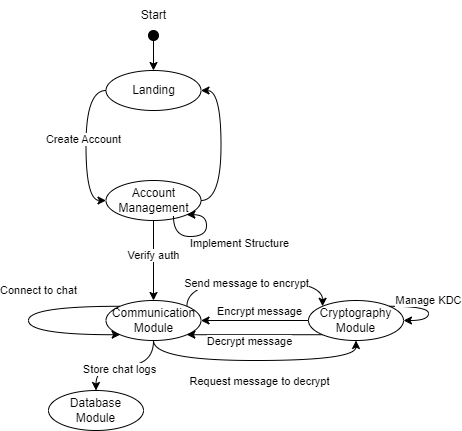
\includegraphics[scale = 0.8]{3A04_D1.png}
\end{center}
% End SubSection

\subsection{User Characteristics}
\label{sub:user_characteristics}
% Begin SubSection
\begin{itemize}
	\item Describe those general characteristics of the intended users of the product including educational level, experience, and technical expertise 
	\item Since there will be many users, you may wish to divide into different user types or personas
%	\item Do not state specific requirements, but rather provide the reasons why certain specific requirements are later specified
\end{itemize}
% End SubSection

\subsection{Constraints}
\label{sub:constraints}
% Begin SubSection
\begin{itemize}
	\item Provide a general description of any constraints that will limit the developer's options
\end{itemize}
% End SubSection

\subsection{Assumptions and Dependencies}
\label{sub:assumptions_and_dependencies}
% Begin SubSection
\begin{itemize}
	\item List any assumptions you made in interpreting what the software being developed is aiming to achieve
	\item List any other assumptions you made that, if it fails to hold, could require you to change the requirements
	%\item List each of the factors that affect the requirements stated in the SRS
	%\item These factors are not design constraints on the software but are, rather, any changes to them that can affect the requirements in the SRS
	\begin{itemize}
		\item \textbf{Example}: An assumption may be that a specific operating system will be available on the hardware designated for the software product. If, in fact, the operating system is not available, the SRS would then have to change accordingly.
	\end{itemize}
\end{itemize}
% End SubSection

\subsection{Apportioning of Requirements}
\label{sub:apportioning_of_requirements}
% Begin SubSection
\begin{itemize}
	\item Identify requirements that may be delayed until future versions of the system
\end{itemize}
% End SubSection

% End Section
\section{Use Case Diagram}
\label{sec:use_case_diagram}
% Begin Section
\begin{itemize}
	\item Provide the use case diagram for the system being developed.
	\item You do not need to provide the textual description of any of the use cases here (these will be specified under "Highlights of Functional Requirements").
%	\item Provide \emph{one} use case diagram for the most important Business Event.
%	\item The text of all use cases will be specified under "Highlights of Functional Requirements"
\end{itemize}
%In this section, select the most important Business Event that your system responds to and give its use case diagram.  Only one use case diagram is needed.  Give a brief textual description of the use case without repeating what is in the scenarios of the corresponding Business Event.

%
%
%
%This section should provide a use case diagram for your application. 
%\begin{enumerate}[a)]
%	\item Each use case appearing in the diagram should be accompanied by a text description. 
%\end{enumerate}
%% End Section

\section{Highlights of Functional Requirements}
\label{sec:functional_requirements}
% Begin Section
\begin{itemize}
	\item Specify all use cases (or other scenarios triggered by other events), organized by Business Event. 
	\item For each Business Event, show the scenario from every Viewpoint. You should have the same set of Viewpoints across all Business Events. If a Viewpoint doesn't participate, write N/A so we know you considered it still. You can choose how to present this - keep in mind it should be easy to follow. 
	\item At the end, combine them all into a Global Scenario.
	%\item Specify the "use cases" (or other triggering events) organized by Business Event. (The Global Scenario is what you might think of as a use case). Be sure to consider Business Events that aren't just triggered by users with goals (e.g. something happens in the environment that your system needs to respond to)
	\item Your focus should be on what the system needs to do, not how to do it. Specify it in enough detail that it clearly specifies what needs to be accomplished, but not so detailed that you start programming or making design decisions.
	\item Keep the length of each use case (Global Scenario) manageable. If it's getting too long, split into sub-cases.
	\item You are \emph{not} specifying a complete and consistent set of functional requirements here. (i.e. you are providing them in the form of use cases/global scenarios, not a refined list). For the purpose of this project, you do not need to reduce them to a list; the global scenarios format is all you need.
	\item Red text below is just to highlight where you need to insert a scenario - don't actually write it all in red.
\end{itemize}

\noindent {\bf Main Business Events:} List out all the main business events you are presenting. If you sub-divided into smaller ones, you don't need to include the smaller ones in this list.\\

\noindent {\bf Viewpoints:} List out all the viewpoints you will be considering.\\

\noindent {\bf Interpretation:} Specify any liberties you took in interpreting business events, if necessary.\\

\begin{enumerate}[{\bf BE1.}]
	\item Business Event Name \#1
		\begin{enumerate}[{\bf VP1.}]
			\item Viewpoint Name \#1 \\
				\textcolor{red}{Insert Scenario Here}
			\item Viewpoint Name \#2 \\
				\textcolor{red}{Insert Scenario Here}
		\end{enumerate}
		{\bf Global Scenario:}\\
		\textcolor{red}{Insert Scenario Here}
	\item Business Event Name \#2
	\begin{enumerate}[{\bf VP1.}]
		\item Viewpoint Name \#1 \\
		\textcolor{red}{Insert Scenario Here}
		\item Viewpoint Name \#2 \\
		\textcolor{red}{Insert Scenario Here}
	\end{enumerate}
	{\bf Global Scenario:}\\
	\textcolor{red}{Insert Scenario Here}
\end{enumerate}

%	Below, we organize by Business Event.
%	\begin{enumerate}[{BE}1.]
%		\item Business Event name
%		\begin{enumerate}[{VP1}.1]
%			\item Viewpoint name \newline
%			\noindent\fbox{%
%				\parbox{0.5\textwidth}{%
%					\begin{itemize}
%						\item {\bf $S_{1}$:} Initial response of the system to the Business Event
%						\item {\bf $E_{1}$:}  Reaction of the environment to $S_{1}$
%						\item {\bf $S_{2}$:}  Response of the system to $E_{1}$
%						\item {\bf $E_{2}$:}  Reaction of the environment to $S_{2}$
%						\item[] $\cdots$
%						\item {\bf $S_{n}$:}  Response of the system to $E_{(n-1)}$
%						\item {\bf $E_{n}$:}  Reaction of the environment to $E_{(n-1)}$
%						\item {\bf $S_{(n+1)}$:} Final response of the system concluding its function regarding the Business Event
%					\end{itemize}
%				}%
%			}
%			\item Viewpoint name\newline
%			\noindent\fbox{%
%				\parbox{0.5\textwidth}{%
%					\begin{itemize}
%						\item {\bf $S_{1}$:} Initial response of the system to the Business Event
%						\item {\bf $E_{1}$:}  Reaction of the environment to $S_{1}$
%						\item {\bf $S_{2}$:}  Response of the system to $E_{1}$
%						\item {\bf $E_{2}$:}  Reaction of the environment to $S_{2}$
%						\item[] $\cdots$
%						\item {\bf $S_{k}$:}  Response of the system to $E_{(k-1)}$
%						\item {\bf $E_{k}$:}  Reaction of the environment to $E_{(k-1)}$
%						\item {\bf $S_{(k+1)}$:} Final response of the system concluding its function regarding the Business Event
%					\end{itemize}
%				}%
%			}
%			\item \dots
%			\item \dots
%			\item \dots
%			\item[\dots]
%		\end{enumerate}	
%		\item[] {\bf Global Scenario of {\it Business Event Name}:} It is the scenario corresponding to the integration of all the above scenarios from the different Viewpoints of the Business Event BE1.\newline
%		\noindent\fbox{%
%			\parbox{0.5\textwidth}{%
%				\begin{itemize}
%					\item {\bf $S_{1}$:} Initial response of the system to the Business Event
%					\item {\bf $E_{1}$:}  Reaction of the environment to $S_{1}$
%					\item {\bf $S_{2}$:}  Response of the system to $E_{1}$
%					\item {\bf $E_{2}$:}  Reaction of the environment to $S_{2}$
%					\item[] $\cdots$
%					\item {\bf $S_{m}$:}  Response of the system to $E_{(m-1)}$
%					\item {\bf $E_{m}$:}  Reaction of the environment to $E_{(m-1)}$
%					\item {\bf $S_{(m+1)}$:} Final response of the system concluding its function regarding the Business Event
%				\end{itemize}
%			}%
%		}	
%		%\end{enumerate}
%		\item Business Event name
%		\begin{enumerate}[{VP1}.1]
%			\item Viewpoint name \newline
%			\noindent\fbox{%
%				\parbox{0.5\textwidth}{%
%					\begin{itemize}
%						\item {\bf $S_{1}$:} Initial response of the system to the Business Event
%						\item {\bf $E_{1}$:}  Reaction of the environment to $S_{1}$
%						\item {\bf $S_{2}$:}  Response of the system to $E_{1}$
%						\item {\bf $E_{2}$:}  Reaction of the environment to $S_{2}$
%						\item[] $\cdots$
%						\item {\bf $S_{n'}$:}  Response of the system to $E_{(n'-1)}$
%						\item {\bf $E_{n'}$:}  Reaction of the environment to $E_{(n'-1)}$
%						\item {\bf $S_{(n'+1)}$:} Final response of the system concluding its function regarding the Business Event
%					\end{itemize}
%				}%
%			}
%			\item Viewpoint name\newline
%			\noindent\fbox{%
%				\parbox{0.5\textwidth}{%
%					\begin{itemize}
%						\item {\bf $S_{1}$:} Initial response of the system to the Business Event
%						\item {\bf $E_{1}$:}  Reaction of the environment to $S_{1}$
%						\item {\bf $S_{2}$:}  Response of the system to $E_{1}$
%						\item {\bf $E_{2}$:}  Reaction of the environment to $S_{2}$
%						\item[] $\cdots$
%						\item {\bf $S_{k'}$:}  Response of the system to $E_{(k'-1)}$
%						\item {\bf $E_{k'}$:}  Reaction of the environment to $E_{(k'-1)}$
%						\item {\bf $S_{(k'+1)}$:} Final response of the system concluding its function regarding the Business Event
%					\end{itemize}
%				}%
%			}
%			\item \dots
%			\item \dots
%			\item \dots
%			\item[\dots]
%		\end{enumerate}	
%		\item[] {\bf Global Scenario of {\it Business Event Name}:} It is the scenario corresponding to the integration of all the above scenarios from the different Viewpoints of the Business Event BE2.\newline
%		\noindent\fbox{%
%			\parbox{0.5\textwidth}{%
%				\begin{itemize}
%					\item {\bf $S_{1}$:} Initial response of the system to the Business Event
%					\item {\bf $E_{1}$:}  Reaction of the environment to $S_{1}$
%					\item {\bf $S_{2}$:}  Response of the system to $E_{1}$
%					\item {\bf $E_{2}$:}  Reaction of the environment to $S_{2}$
%					\item[] $\cdots$
%					\item {\bf $S_{m'}$:}  Response of the system to $E_{(m'-1)}$
%					\item {\bf $E_{m'}$:}  Reaction of the environment to $E_{(m'-1)}$
%					\item {\bf $S_{(m'+1)}$:} Final response of the system concluding its function regarding the Business Event
%				\end{itemize}
%			}%
%		}		
%	\end{enumerate}

%End Section

\section{Non-Functional Requirements}
\label{sec:non-functional_requirements}


\begin{itemize}
	\item For each non-functional requirement, provide a justification/rationale for it.\\
	{\bf Example:} \\
	SC1. \emph{The device should not explode in a customer’s pocket.}\\
	{\bf Rationale:} Other companies have had issues with the batteries they used in their phones randomly exploding [insert citation]. This causes a safety issue, as the phone is often carried in a person's hand or pocket.	
	\item If you need to make a guess because you couldn't really talk to stakeholders, you can say "We imagined stakeholders would want...because..."
	\item Each requirement should have a unique label/number for it.
	\item In the list below, if a particular section doesn't apply, just write N/A so we know you considered it.
\end{itemize}

% Begin Section
\subsection{Look and Feel Requirements}
\label{sub:look_and_feel_requirements}
% Begin SubSection

\subsubsection{Appearance Requirements}
\label{ssub:appearance_requirements}
% Begin SubSubSection
\begin{enumerate}[{LF-A}1. ]
	\item 
\end{enumerate}
% End SubSubSection

\subsubsection{Style Requirements}
\label{ssub:style_requirements}
% Begin SubSubSection
\begin{enumerate}[{LF-S}1. ]
	\item 
\end{enumerate}
% End SubSubSection

% End SubSection

\subsection{Usability and Humanity Requirements}
\label{sub:usability_and_humanity_requirements}
% Begin SubSection

\subsubsection{Ease of Use Requirements}
\label{ssub:ease_of_use_requirements}
% Begin SubSubSection
\begin{enumerate}[{UH-EOU}1. ]
	\item 
\end{enumerate}
% End SubSubSection

\subsubsection{Personalization and Internationalization Requirements}
\label{ssub:personalization_and_internationalization_requirements}
% Begin SubSubSection
\begin{enumerate}[{UH-PI}1. ]
	\item 
\end{enumerate}
% End SubSubSection

\subsubsection{Learning Requirements}
\label{ssub:learning_requirements}
% Begin SubSubSection
\begin{enumerate}[{UH-L}1. ]
	\item 
\end{enumerate}
% End SubSubSection

\subsubsection{Understandability and Politeness Requirements}
\label{ssub:understandability_and_politeness_requirements}
% Begin SubSubSection
\begin{enumerate}[{UH-UP}1. ]
	\item 
\end{enumerate}
% End SubSubSection

\subsubsection{Accessibility Requirements}
\label{ssub:accessibility_requirements}
% Begin SubSubSection
\begin{enumerate}[{UH-A}1. ]
	\item 
\end{enumerate}
% End SubSubSection

% End SubSection

\subsection{Performance Requirements}
\label{sub:performance_requirements}
% Begin SubSection

\subsubsection{Speed and Latency Requirements}
\label{ssub:speed_and_latency_requirements}
% Begin SubSubSection
\begin{enumerate}[{PR-SL}1. ]
	\item 
\end{enumerate}
% End SubSubSection

\subsubsection{Safety-Critical Requirements}
\label{ssub:safety_critical_requirements}
% Begin SubSubSection
\begin{enumerate}[{PR-SC}1. ]
	\item 
\end{enumerate}
% End SubSubSection

\subsubsection{Precision or Accuracy Requirements}
\label{ssub:precision_or_accuracy_requirements}
% Begin SubSubSection
\begin{enumerate}[{PR-PA}1. ]
	\item 
\end{enumerate}
% End SubSubSection

\subsubsection{Reliability and Availability Requirements}
\label{ssub:reliability_and_availability_requirements}
% Begin SubSubSection
\begin{enumerate}[{PR-RA}1. ]
	\item 
\end{enumerate}
% End SubSubSection

\subsubsection{Robustness or Fault-Tolerance Requirements}
\label{ssub:robustness_or_fault_tolerance_requirements}
% Begin SubSubSection
\begin{enumerate}[{PR-RFT}1. ]
	\item 
\end{enumerate}
% End SubSubSection

\subsubsection{Capacity Requirements}
\label{ssub:capacity_requirements}
% Begin SubSubSection
\begin{enumerate}[{PR-C}1. ]
	\item 
\end{enumerate}
% End SubSubSection

\subsubsection{Scalability or Extensibility Requirements}
\label{ssub:scalability_or_extensibility_requirements}
% Begin SubSubSection
\begin{enumerate}[{PR-SE}1. ]
	\item 
\end{enumerate}
% End SubSubSection

\subsubsection{Longevity Requirements}
\label{ssub:longevity_requirements}
% Begin SubSubSection
\begin{enumerate}[{PR-L}1. ]
	\item 
\end{enumerate}
% End SubSubSection

% End SubSection

\subsection{Operational and Environmental Requirements}
\label{sub:operational_and_environmental_requirements}
% Begin SubSection

\subsubsection{Expected Physical Environment}
\label{ssub:expected_physical_environment}
% Begin SubSubSection
\begin{enumerate}[{OE-EPE}1. ]
	\item 
\end{enumerate}
% End SubSubSection

\subsubsection{Requirements for Interfacing with Adjacent Systems}
\label{ssub:requirements_for_interfacing_with_adjacent_systems}
% Begin SubSubSection
\begin{enumerate}[{OE-IA}1. ]
	\item 
\end{enumerate}
% End SubSubSection

\subsubsection{Productization Requirements}
\label{ssub:productization_requirements}
% Begin SubSubSection
\begin{enumerate}[{OE-P}1. ]
	\item 
\end{enumerate}
% End SubSubSection

\subsubsection{Release Requirements}
\label{ssub:release_requirements}
% Begin SubSubSection
\begin{enumerate}[{OE-R}1. ]
	\item 
\end{enumerate}
% End SubSubSection

% End SubSection

\subsection{Maintainability and Support Requirements}
\label{sub:maintainability_and_support_requirements}
% Begin SubSection

\subsubsection{Maintenance Requirements}
\label{ssub:maintenance_requirements}
% Begin SubSubSection
\begin{enumerate}[{MS-M}1. ]
	\item 
\end{enumerate}
% End SubSubSection

\subsubsection{Supportability Requirements}
\label{ssub:supportability_requirements}
% Begin SubSubSection
\begin{enumerate}[{MS-S}1. ]
	\item 
\end{enumerate}
% End SubSubSection

\subsubsection{Adaptability Requirements}
\label{ssub:adaptability_requirements}
% Begin SubSubSection
\begin{enumerate}[{MS-A}1. ]
	\item 
\end{enumerate}
% End SubSubSection

% End SubSection

\subsection{Security Requirements}
\label{sub:security_requirements}
% Begin SubSection

\subsubsection{Access Requirements}
\label{ssub:access_requirements}
% Begin SubSubSection
\begin{enumerate}[{SR-AC}1. ]
	\item User must be logged into the application to access any information.
	\\\textbf{Rationale:} This is to ensure that only users that have verified their credentials have access to any potentially sensitive information or features.
	\item User must be a part of the company verified list.
	\\\textbf{Rationale:} For a user to join any chats or \textcolor{red}{announcement boards} they must be a verified member of the company that oversees the chats.
	\item User must not have access to ant chats, \textcolor{red}{files or announcements} that they do not belong to.
	\\\textbf{Rationale:} To maintain the secure aspect of the application, only users that belong to certain chats, \textcolor{red}{files or announcements} may view them.
	\item User must consent to have their location being used.
	\\\textbf{Rationale:} To ensure that the user is within a \textcolor{red}{verified geolocation}, the app needs permission to use their GPS location to determine if the location is verified.
	\item User must consent to have their biometric data being used.
	\\\textbf{Rationale:} To utilize \textcolor{red}{biometric data for effective two-factor authentication}, the app needs permission to use the biometric data to determine if the user is who they say they are. 
\end{enumerate}
% End SubSubSection

\subsubsection{Integrity Requirements}
\label{ssub:integrity_requirements}
% Begin SubSubSection
\begin{enumerate}[{SR-INT}1. ]
	\item The system will use an industry accepted end-to-end symmetric-key cryptosystem algorithm.
	\\\textbf{Rationale:} To ensure that the messages being sent back and forth are not being modified in the middle, an end-to-end encryption is necessary. The algorithm to be used will be one of the industry standard algorithms (AES, 3-DES) [8].
	\item Chat logs will be stored separately from the rest of the system.
	\\\textbf{Rationale:} To ensure that the chat logs are not tampered with, they will be stored on a database that is separate from the system that only admins have access to.
	\item Users should not change their name unless company allows it.
	\\\textbf{Rationale:} To verify that users know who they are chatting to, users should not be allowed to change their name unless given permission by the company.

\end{enumerate}
% End SubSubSection

\subsubsection{Privacy Requirements}
\label{ssub:privacy_requirements}
% Begin SubSubSection
\begin{enumerate}[{SR-P}1. ]
	\item The application will adhere to the Google Play Developer Distribution Agreement.
	\\\textbf{Rationale:} As this app is going to be developed for android, adhering to the GPDDA is a step to ensure that privacy is being kept [9].
	\item Personal information of users should not be displayed to anyone outside of themselves.
	\\\textbf{Rationale:} To keep information such as age, gender, an employees department, etc. private, this information should not be displayed to those they are chatting to.
	\item Notifications should not display message content.
	\\\textbf{Rationale:} To maintain the purpose of secure communication, notifications should not contain sensitive information, and rather have a message similar to “you have a notification from VanklComm, you have 8 unread messages”.

\end{enumerate}
% End SubSubSection

\subsubsection{Audit Requirements}
\label{ssub:audit_requirements}
% Begin SubSubSection
\begin{enumerate}[{SR-AU}1. ]
	\item The app must comply with company guidelines for auditing employee chats.
	\\\textbf{Rationale:} To allow for the company to regulate the chats that their employee’s send, the app must provide a way for them to audit effectively. 
\end{enumerate}
% End SubSubSection

\subsubsection{Immunity Requirements}
\label{ssub:immunity_requirements}
% Begin SubSubSection
\begin{enumerate}[{SR-IM}1. ]
	\item Verify with the KDC that the user is authorized.
	\\\textbf{Rationale:} To protect against malware or bad actors, only users authorized by the KDC may use the app.
\end{enumerate}
% End SubSubSection

% End SubSection

\subsection{Cultural and Political Requirements}
\label{sub:cultural_and_political_requirements}
% Begin SubSection

\subsubsection{Cultural Requirements}
\label{ssub:cultural_requirements}
% Begin SubSubSection
\begin{enumerate}[{CP-C}1. ]
	\item No offensive imagery will be used in the composition of the app.
	\\\textbf{Rationale:} To make the app a safe space for all users, any imagery that is known to be offensive to any group of people must be erased from the app.
	\item The app will not send messages that contain inappropriate words.
	\\\textbf{Rationale:} Using Google’s Word list [10] the use of inappropriate words will not be tolerated.
	\item Users can report hateful and/or abusive language to the admin.
	\\\textbf{Rationale:} In order to maintain the safety of users, any inappropriate messages not caught by the word list can be reported by a user.

\end{enumerate}
% End SubSubSection

\subsubsection{Political Requirements}
\label{ssub:political_requirements}
% Begin SubSubSection
\begin{enumerate}[{CP-P}1. ]
	\item Users may only send direct messages to those who they are authorized to message.
	\\\textbf{Rationale:} A low level factory worker should not be messaging the CEO unless they have permission granted to do so.
	\item Employees may send a message request to those they are unauthorized to message.
	\\\textbf{Rationale:} Similar to Facebook Messenger, if an employee is unauthorized, their message should go to a separate inbox that does not flood the receiver, but they can check to see the request.
\end{enumerate}
% End SubSubSection

% End SubSection

\subsection{Legal Requirements}
\label{sub:legal_requirements}
% Begin SubSection

\subsubsection{Compliance Requirements}
\label{ssub:compliance_requirements}
% Begin SubSubSection
\begin{enumerate}[{LR-COMP}1. ]
	\item The app will be SMS compliant [11].
	\\\textbf{Rationale:} To follow the law, the app must be SMS compliant as it is technically a text messaging service.
\end{enumerate}
% End SubSubSection

\subsubsection{Standards Requirements}
\label{ssub:standards_requirements}
% Begin SubSubSection
\begin{enumerate}[{LR-STD}1. ]
	\item The app will comply with the Android App Quality Standards [12].
	\\\textbf{Rationale:} To maintain good standards, the app will follow the standards given by Android.
\end{enumerate}
% End SubSubSection

% End SubSection

% End Section

\appendix
\section{Division of Labour}
\label{sec:division_of_labour}
% Begin Section
Include a Division of Labour sheet which indicates the contributions of each team member. This sheet must be signed by all team members.
% End Section

%\newpage
%\section*{IMPORTANT NOTES}
%\begin{itemize}
%	\item Be sure to include all sections of the template in your document regardless whether you have something to write for each or not
%	\begin{itemize}
%		\item If you do not have anything to write in a section, indicate this by the \emph{N/A}, \emph{void}, \emph{none}, etc.
%	\end{itemize}
%	\item Uniquely number each of your requirements for easy identification and cross-referencing
%	\item Highlight terms that are defined in Section~1.3 (\textbf{Definitions, Acronyms, and Abbreviations}) with \textbf{bold}, \emph{italic} or \underline{underline}
%	\item For Deliverable 1, please highlight, in some fashion, all (you may have more than one) creative and innovative features. Your creative and innovative features will generally be described in Section~2.2 (\textbf{Product Functions}), but it will depend on the type of creative or innovative features you are including.
%\end{itemize}


\end{document}
%------------------------------------------------------------------------------